\documentclass[a4paper,parskip,DIV=10,11pt]{scrbook}

%\usepackage{german}
\usepackage[T3,T1]{fontenc}
\usepackage[utf8]{inputenc}
\usepackage{amsmath}
\usepackage{amsfonts}
\usepackage{amssymb}
\usepackage{mathtools}
\usepackage{faktor}
\usepackage{nicefrac}
\usepackage{listings}
\usepackage{enumerate}
\usepackage{dsfont}
\usepackage{remreset}
\usepackage{booktabs}
\usepackage{lettrine}
%\usepackage{txfonts}
\usepackage{varioref}
\usepackage{multirow}
\usepackage{rotating}
\usepackage{cancel}
\usepackage[pdfauthor={Joachim Breitner}]{hyperref}
\usepackage[capitalise]{cleveref}
\usepackage{tikz}
\usetikzlibrary{snakes,arrows,shapes}
% \usetikzlibrary{automata}
% \usetikzlibrary{decorations}
% \usetikzlibrary{snakes}
\usepackage{microtype}
\usepackage{framed}
\usepackage{caption}
\usepackage[normalem]{ulem}

%\usepackage{tipa} Causes warnings with \iff
\DeclareTextSymbol\textlambda{T3}{171}           % Lambda
\DeclareTextSymbolDefault\textlambda{T3}

\usepackage{isabelle,isabellesym}
\isabellestyle{it}

\usepackage[numbers,square]{natbib}
\bibliographystyle{amsplain}

% URLstyle
\urlstyle{rm}

% for \autoref
\newcommand{\examplename}{Example}
\newcommand{\lemmaname}{Lemma}
\newcommand{\remarkname}{Remark}
\newcommand{\corollaryname}{Corollary}
\newcommand{\definitionname}{Definition}
\newcommand{\algocflinename}{Algorithm}
\newcommand{\AlgoLineautorefname}{line}
\renewcommand{\chapterautorefname}{Chapter}
\renewcommand{\sectionautorefname}{Section}
\renewcommand{\subsectionautorefname}{Section}

% for \cref
\crefname{algocf}{Algorithm}{Algorithms}
\crefname{figure}{Figure}{Figure}

% vref settings
\vrefwarning
\def\reftextfaceafter {\unskip}%
\def\reftextfacebefore{\unskip}%
\def\reftextafter     {on the \reftextvario{following}{next} page}%
\def\reftextbefore    {on the \reftextvario{preceding}{previous} page}%
\def\reftextcurrent   {\unskip}%

% titlesec
\usepackage{titlesec}
\titleformat{\chapter}[display]
	{\sectfont\Large\filcenter}
	{\titlerule%[1pt]%
	 \vspace{1pt}%
	 \titlerule%
	 %\vspace{.4pc}%
	 \LARGE\MakeUppercase{\chaptertitlename} \thechapter}
	{1pc}
	{\titlerule
	 \vspace{1pc}%
	 \Huge}
% \titleformat{\chapter}[display]
% 	{\sectfont\Large}
% 	{%\titlerule%[1pt]%
% 	 %\vspace{1pt}%
% 	 %\titlerule%
% 	 %\vspace{.4pc}%
% 	 \LARGE{\chaptertitlename} \thechapter}
% 	{1pc}
% 	{%\titlerule
% 	 %\vspace{1pc}%
% 	 \sectfont%
% 	 \Huge}

%\pagestyle{headings}

% get rid of fourier fontenc warnings
% from http://newsgroups.derkeiler.com/Archive/Comp/comp.text.tex/2006-01/msg00679.html
\makeatletter
\let\my@@font@warning\@font@warning
\let\@font@warning\@font@info
\makeatother
%
\usepackage{mathpazo}
%\usepackage{fourier}
%\usepackage[math]{iwona}
%\usepackage{ccfonts}
%\usepackage{arev}
%\usepackage[garamond]{mathdesign}
%\usepackage{pxfonts}
%
\makeatletter
\let\@font@warning\my@@font@warning
\makeatother 

% Palatino: 5% mehr Zeilendurchschuss (laut KOMA-skript)
\linespread{1.05}

% Satzspiegel neu berechen
\recalctypearea

% Figures unabhängig vom Kapitel zählen
\makeatletter
\@removefromreset{figure}{chapter}
\renewcommand{\thefigure}{\arabic{figure}}
\@removefromreset{table}{chapter}
\renewcommand{\thetable}{\arabic{table}}
\makeatother

% Disable single lines at the start of a paragraph (Schusterjungen)
\clubpenalty = 10000
%
% Disable single lines at the end of a paragraph (Hurenkinder)
\widowpenalty = 10000 \displaywidowpenalty = 10000

% Remove skip between caption and figure.
\captionsetup[figure]{skip=0pt}

% listings
\lstset{language=Haskell
	,flexiblecolumns=True
	,columns=fullflexible
	,texcl=true
	,escapechar=!
	,basicstyle=\sffamily
	,stringstyle=\itshape
	,showstringspaces=false
	,literate={->}{$\to\,\,$}2 {→}{$\to\,\,$}2 {\\}{\textlambda}1
	}

% inputenc stuff
\DeclareUnicodeCharacter{03BB}{\textlambda}

% FrameSep default
\setlength{\FrameSep}{2pt}

% Float placement
%\renewcommand{\topfraction}{.95}
%\renewcommand{\bottomfraction}{.7}
%\renewcommand{\textfraction}{.05}
\renewcommand{\floatpagefraction}{.60}
%\renewcommand{\dbltopfraction}{.66}
%\renewcommand{\dblfloatpagefraction}{.66}
\setcounter{topnumber}{1}
\setcounter{bottomnumber}{1}


\newcommand{\C}{\mathcal C}
\newcommand{\F}{\mathcal F}
\newcommand{\PR}{\mathcal {PR}}
\newcommand{\A}{\mathcal A}


\newcommand{\aC}{\widehat{\mathcal C}}
\newcommand{\aF}{\widehat{\mathcal F}}
\newcommand{\aPR}{\widehat{\mathcal {PR}}}
\newcommand{\aA}{\widehat{\mathcal A}}

\newcommand{\N}{\mathds N}
\newcommand{\da}{\coloneqq}
\newcommand{\id}{\text{id}}
\newcommand{\fix}{\text{fix}}

\hyphenation{Karls-ruhe}

\author{Joachim Breitner}
\title{Control Flow in Functional Languages}
\subtitle{Formally taming lambdas}

\begin{document}
%\KOMAoptions{twoside=false}
\begin{titlepage}
\centering
\makeatletter
\textsc{\Large{Karlsruher Institut für Technologie}}\\
\vspace{.5em}
\textsc{\Large{Fakultät für Informatik}} \\
\vspace{4em}
{\Large \@author} \\
\vspace{2em}
{\large Student Research Project}\\
\vspace{2.5em}
{\sectfont\huge \@title }\\
\vspace{2em}
{\sectfont\Large \@subtitle }\\
% \vfill
% \begin{tikzpicture}[auto]
% \end{tikzpicture} \\
\vfill
Supervisors: \\
Prof. Dr. Gregor Snelting \\
Andreas Lochbihler \\
\vspace{2em}
{\large \@date }
\makeatother
\end{titlepage}
%\KOMAoptions{twoside=true}


\chapter*{Abstract}

\lettrine I{n} his dissertation\cite{Shivers}, Olin Shivers introduces a concept of control flow graphs for functional languages, provides an algorithm to statically derive a safe approximation of the control flow graph and proves this algorithm correct. In this student research project, Shiver’s algorithms and proofs are formalized using the theorem prover system Isabelle.


\tableofcontents

\chapter{Introduction}

\lettrine C{ontrol} Flow Analysis plays an important role in compiler construction as well as in security analysis. Having the latter case in mind, Daniel Wasserrab provides a formally verified framework acting on an abstract and language-independent control flow graph in his dissertation\citep{wasserrab}. This framework has been instantiated for programs written in either a simple toy imperative language, a subset of C++ or the Java-like language Jinja\citep{jinja}.

All these programming languages are imperative. Therefore, we are interested in its applicability to functional languages. This requires a notion notion of a control flow graph for a functional programs. In 1991, Olin Shivers defined such a control flow graph and develops a statical analysis algorithm to calculate it. Later research about functional control flow is often based on his definition.

To be able to connect to Wasserrab’s framework, the definitions and algorithms of Shivers need to be formalized in the theorem prover system Isabelle. This is the main goal of this project. The actual connection will be treated only theoretically.

This document starts with a concise overview of Shivers’ approach in \cref{chapshivers}. Then we explain the prototype in Haskell (\cref{chaphaskell}) as well as the formalization in Isabelle (\cref{chapisabelle}), stating where it differs from the original. We motivate some of the more interesting choices in the formalization, such as the use of \isa{HOLCF}. Some lemmas took several failed or unsatisfying attempts, which we do not hush up. We took special care to make the appearance of the documents generated by Isabelle as similar to the original as possible. \cref{seclayout} presents the tricks used to that end. \cref{chapslicing} explains the how these results could be connected to Wasserrab’s framework.

A total of 3625 lines of Isabelle code (including commentary) and 890 lines of Haskell code (include 199 lines of commentary) were written.


% \vfill
% \lettrine[nindent=1ex]I{} owe sincere thanks to Dr.\ Gabriela Schmithüsen, under whose guidance this thesis was created. She was always generous with time, advice, regular proof-reading, ideas and inspiration.
% 
% Moreover, I wish to thank Mareike Schmidtobreick and Pascal Maillard for proof-reading the final work.

\chapter{Taming Lambdas}
\label{chapshivers}

\lettrine F{unctional} languages, i.e.\ programming languages that treat computations, including their context, as first class citizens, are harder to tackle by control flow analysis than imperative languages. For the latter, a function call names the function that will be called and a statical analysis can easily trace the control flow at that point. In functional languages, the callee can be a variable which, in turn, can contain any computation that was stored somewhere else in the program.

Additionally, such a stored computation is a \textit{closure}, i.e.\ contains the currently valid variable bindings. Therefore, a variable can have more than one current value at any given point in the program execution, where different closures see different values. This is an additional issue when trying to statically make statements about a function program’s control flow.

Shivers approaches this problem in his 1991 Ph.D.\ thesis, subtitled “taming lambdas”. He defines an exemplary functional language in \textit{continuation-passing style} (CPS). CPS means that the return value of functions can not return, but rather passed on to a continuation function, which has to be given as an argument. Consider for example the following code :
\begin{lstlisting}[language=Haskell]
main = print ((x + y) * (z - w))
\end{lstlisting}
In continuation-passing style, the operations \lstinline!+!, \lstinline!*!, \lstinline!-! and \lstinline!print! all take a continuation argument, and the \lstinline!main! function is being passed a top-level continuation: 
\begin{lstlisting}[language=Haskell]
main c = + x y (\xy. - z w (\zw. * xy zw (\prod. print prod c)))
\end{lstlisting}

\section{Syntax}

\begin{figure}
\begin{framed}
\begin{align*}
\text{PR} &\Coloneqq \text{LAM} \\
\text{LAM} &\Coloneqq (\lambda\ (v_1\ldots v_n)\ c) && [v_i\in \text{VAR},\, c\in\text{CALL}] \\
\text{CALL} &\Coloneqq (f\ a_1 \ldots a_n) && [f\in \text{FUN},\, a_i\in\text{ARG}] \\
&\phantom{\strut\Coloneqq\strut} (\text{\texttt{letrec}}\ ((f_1\ l_1)\ldots)\ c) && [f_i\in \text{VAR},\,l_i\in\text{LAM},\,c\in\text{CALL}] \\
\text{FUN} &\Coloneqq \text{LAM} + \text{REF} + \text{PRIM} \\
\text{ARG} &\Coloneqq \text{LAM} + \text{REF} + \text{CONST} \\
\text{REF} &\Coloneqq \text{VAR} \\
\text{VAR} &\Coloneqq \{\text{\texttt{x},\texttt{y},\texttt{foo},}\ldots\} \\
\text{CONST} &\Coloneqq \{\text{\texttt{3},\texttt{\#f},}\ldots\} \\
\text{PRIM} &\Coloneqq \{\text{\texttt{+},\texttt{if},\texttt{test-integer},}\ldots\} \\
\text{LAB} &\Coloneqq \{l_i,r_i,c_i,ic_p^j\ldots\}
\end{align*}
\end{framed}
\caption{CPS syntax}
\label{fig:syntax}
\end{figure}

The syntax definition is given in \vref{fig:syntax}. A Program (PR) is a lambda expression. Lambda expressions (LAM) abstract a call. Calls (CALL) either call a function with the given argument list or binds lambdas to names in a possibly mutually recursive fashion. Function values (FUN) can be lambda expressions, references to variables or primitive operations, while in argument positions (ARG), primitive operations are disallowed and constant expressions are allowed. References to variables (REF) name the referenced variable. There is a set of variable names (VAR). Constants (CONST) are either integers or \#f for a false value. A number of primitive operations (PRIM) are defined.

Although not given explicitly, every lambda, call, constant, variable reference and primitive operation is tagged with a unique label from the set LAB. These can be thought of as positions in the program source – for our purpose they are just an abstract set. Also we assume that programs are alphatised, i.e.\ each variable name $v$ is bound at exactly one position, whose label is given by $\text{\textit{binder}}\ v$. Additional \textit{internal labels} are added to this set for primitive operations, representing the internal call sites. For example the \texttt{if} primitive operation is being passed two continuation that might be called, one for the true case and one for the false case. Therefore, two internal labels are associated with this primitive operation.

\section{Standard Semantics}
\begin{figure}
\setlength{\FrameSep}{0pt}
\begin{framed}
\begin{align*}
\text{Bas} &= \mathds Z + \{\text{false}\} 
						& \PR &\colon \text{PR} \rightharpoonup \text{Ans} \\
\text{Clo} &= \text{LAM} \times \text{BEnv} 
						& \A &\colon \text{ARG}\cup\text{FUN} \to \text{BEnv} \to \text{VEnv} \to \text{D} \\
\text{Proc} &= \text{Clo} + \text{PRIM} + \{\text{\textit{stop}}\} 
						& \C &\colon \text{CALL}\to \text{BEnv} \to \text{VEnv} \to \text{CN} \rightharpoonup \text{Ans} \\
\text{D} &= \text{Bas} + \text{Proc}
						& \F &\colon \text{Proc}\to \text{D}^* \to \text{VEnv} \to \text{CN} \rightharpoonup \text{Ans} \\
\text{CN} &= \text{\textit{(contours)}} \\
\text{BEnv} &= \text{LAB} \rightharpoonup \text{CN} \\
\text{VEnv} &= (\text{VAR}\times\text{CN}) \rightharpoonup \text{D}\\
\text{Ans} &= (\text D + \{\text{\textit{error}}\})_\bot
\end{align*}
\end{framed}
\caption{CPS semantics domains}
\label{fig:semdoms}
\end{figure}


For this language, Shivers gives a denotational semantics for the above language, that is a partial function $\PR$ from the set of programs to the set of integers with an additional element indicating run-time errors. Following the structure of the syntax tree, he defines functions $\C$, $\F$ and $\A$ that evaluate call expressions, apply arguments to procedures and evaluate argument expressions, respectively. Their domains and ranges are given in \vref{fig:semdoms}. The rather lengthy equations of their definitions are omitted here.

Semantic values (D) can either be basic values (Bas) which consist of the integers plus the value representing false, or a procedure. Procedures (Proc) again are either a closure, which is a lambda expression bundled with a context, a primitive operation or \textit{stop}.

The special value \textit{stop} is the continuation initially passed to the program. When this is eventually called, either in a CALL expression or as the continuation of a primitive operation, the evaluation comes to an halt and the argument to stop is the result of the evaluation. If a runtime error occurs (wrong number of arguments, callee not a procedure, undefined variable lookup), \textit{error} is returned.

The semantics functions are partial functions, indicated by the harpoon instead of the arrow and by the $\bot$ annotation of the set Ans of answer values. Functional programs are Turing-complete and therefore possibly non-terminating. For such programs, the semantics is defined to return $\bot$.

The evaluation context needs to be passed along the semantics functions and closures value need to encapsulate the context at the time the lambda expression is evaluated to a closure. The context information is separated into two maps here: The global \textit{variable environment} (VEnv) and the lexical \textit{contour environment} (or binding environment, BEnv, in the following usually denoted by $\beta$). The variable environment can store multiple values for each variable name. These are differentiated by a \textit{contour number} from the set CN. These can be thought of time stamps which are increased in every evaluation step. When a variable is bound to a new value, it is stored in the variable environment with the current contour number. The contour environment tells for each binding position (lambda or letrec expression) which contour counter is to be used when looking up a variable from that binding. By storing the contour environment within a closure and using it when evaluating the call inside the closure, the correct value for each variable binding is accessed.

The set CN of contours is not given explicitly here. Instead, we will treat it abstractly and only state the properties we expect from this set: There needs to be an initial contour $b_0$ and a function $nb \colon \text{CN} \to \text{CN}$ which generates a new contour. The set of contours is partially ordered and if $b$ is greater or equal than all allocated contours, then $nb\ b$ is strictly greater than all allocated contours. It is easy to see that the natural numbers with $b_0 = 0$ and $nb\ b = \text{Suc}\ b$ fulfill the requirements, but in the later proofs it will be convenient to choose other sets containing more information. 

\section{Exact nonstandard semantics}

\begin{figure}
\begin{align*}
\C\ (c:(f\ a_1\ldots a_n))\ \beta\ ve\ b &= 
\begin{cases}
[], & f' \notin \text{Proc} \\
(\F\ f'\ av\ ve\ b' )[(c,\beta) \mapsto f'], &\text{otherwise}
\end{cases}\\
&\phantom{\strut=\strut}\text{where } f' = \A\ f\ \beta\ ve \\
&\phantom{\strut=\text{where }} av_i = \A\ a_i\ \beta\ ve \\
\end{align*}
\vspace{-1em}
\caption{The exact nonstandard semantics for a call expression}
\label{fig:callsem}
\end{figure}

At the moment we are not so much interested in the value a program returns but rather the calls that occur while evaluating the program. To that end the standard semantics introduced in the previous section is altered to calculate the \textit{call cache}. This is a partial map from call-site/contour-environment pairs to procedures. We therefore modify the domains of the semantics in \vref{fig:semdoms} as follows:
\begin{align*}
\text{CCache} &= (\text{LAB}\times\text{BEnv}) \rightharpoonup \text{Proc}\\
\text{Ans} &= \text{CCache}
\end{align*}

The semantics function definitions are extended to record the calls as they happen \vref{fig:callsem} shows exemplary the equation of $\C$ for a call expression $(f\ a_1\ldots a_n)$ with label $c$. If the syntactic value $f$ is evaluated to a procedure $f'\in \text{Proc}$, evaluation continues by applying $\F$ to $f'$ and the arguments. This returns a call cache, which is amended by the entry $(c,\beta) \mapsto f'$ to reflect the current call before the updated call cache is returned by $C$.

This semantics evaluates the program in full, just like the standard semantics, and is therefore unsuitable to be used in a static analysis. But it is the theoretic ideal that a statically calculated call cache will be compared against.

\section{Abstract nonstandard semantics}

Shivers then proceeds to define a nonstandard semantics that can be calculated statically. The trade off is that the call cache obtained now is just an approximation to the exact call cache, i.e.\ any possible call in the exact call cache will also be in the abstract call cache. The converse does not need to hold.

\begin{figure}
\setlength{\FrameSep}{0pt}
\begin{framed}
\begin{align*}
\widehat{\text{Clo}} &= \text{LAM} \times \widehat{\text{BEnv}}
						& \aPR &\colon \text{PR} \rightharpoonup \widehat{\text{Ans}} \\
\widehat{\text{Proc}} &= \widehat{\text{Clo}} + \text{PRIM} + \{\text{\textit{stop}}\} 
						& \aA &\colon \text{ARG}\cup\text{FUN} \to \widehat{\text{BEnv}} \to \widehat{\text{VEnv}} \to \widehat{\text{D}} \\
\widehat{\text{D}} &= \mathcal P(\widehat{\text{Proc}})
						& \aC &\colon \text{CALL}\to \widehat{\text{BEnv}} \to \widehat{\text{VEnv}} \to \widehat{\text{CN}} \rightharpoonup \widehat{\text{Ans}} \\
\widehat{\text{CN}} &= \text{\textit{(contours, finite)}} 
						& \aF &\colon \widehat{\text{Proc}}\to \widehat{\text{D}}^* \to \widehat{\text{VEnv}} \to \widehat{\text{CN}} \rightharpoonup \widehat{\text{Ans}} \\
\widehat{\text{BEnv}} &= \text{LAB} \rightharpoonup \widehat{\text{CN}} \\
\widehat{\text{VEnv}} &= (\text{VAR}\times \widehat{\text{CN}}) \rightharpoonup \widehat{\text{D}} \\
\widehat{\text{CCache}} &= (\text{LAB} \times \widehat{\text{BEnv}}) \to \widehat{\text{D}} \\
\widehat{\text{Ans}} &= \widehat{\text{CCache}}
\end{align*}
\end{framed}
\caption{CPS semantics domains}
\label{fig:abssemdoms}
\end{figure}

The abstract semantics $\aPR$ will run the program no longer in full detail. It will not keep track of actual values computed and conditional branches taken. Instead, it assumes that every branch of an \texttt{if} statement is possibly taken. Semantic values are now sets of possible procedures. \vref{fig:abssemdoms} gives the domains of the abstract semantics functions. 

After removing the plain values from our semantics domains, the remaining would all be finite – if  $\widehat{\text{CN}}$ were finite. This is the main trick to obtain a computable abstract semantics. If $\widehat{\text{CN}}$ is finite, there are only finitely many possible closures, procedures, binding environment, variable environments and call caches, and our function becomes computable.

Again, the choice of the set $\widehat{\text{CN}}$ is not fixed. Possible choices include a singleton set, resulting in “0th-order Control Flow Analysis” (0CFA) or the set of lambdas representing the call site a lambda was called from, resulting in 1st-order Control Flow Analysis (1CFA). The more information we store in the abstract contour counters, the more detailed our analysis will be, but also more expensive to calculate.

Because semantic values $\widehat{\text{D}}$ are now sets of procedures, when evaluating a call expression $(f\ a_1\ldots a_n)$, there is a set of possible procedure that $f$ can evaluate to, and $\aF$ will be called for each of them. The resulting call caches need to be joined using pointwise set union. Similarly, the continuations of primitive operations are sets of procedures, for all of which $\aF$ is called and the result is joined again.

\section{Main results}

The main results about these semantics functions are stated and shown in Shivers’ dissertation:
\begin{enumerate}
\item The call cache returned by the exact semantics is indeed a partial map,
\item the abstract semantics approximate the exact semantics and
\item the abstract semantics is computable.
\end{enumerate}

But before starting to prove these results, Shivers establishes that the recursive definitions he gave for $\F$ and $\C$ (and by analogy, $\aF$ and $\aC$) are sound. He proceeds in the standard way of turning a recursive definitions $f = F f$ for a function $f\in X$, where $X$ is a function space with a chain-complete partial order, into a functional $F\colon X \to X$. $F$ is then shown to be continuous and therefore has a least fixed point, which is used then defined to be $f$.
  

The need to show that the result of $\PR$ is a partial map arises from the fact that, for an easier proof of continuity, Shivers changes the answer domain to be
\[
\text{Ans} = \mathcal P( (\text{LAB}\times\text{BEnv}) \times \text{Proc}).
\]
The actual proof is only outlined.

In contrast, the proof that $\aPR$ safely approximates $\PR$ is given in full detail. For any of the types Proc, D, $\text{D}^*$, BEnv, VEnv, CN and CCache, he defines an abstraction function (written $|\cdot|$) from the exact type to the corresponding abstract type. He also defines partial orders on the abstract types (written $\cdot \lessapprox \cdot$), expressing that one value is more specific than another value. The main result is then
\begin{quote}
\textbf{Theorem 6}: For any program $l$, call site label $c$ and binding environment $\beta$, we have
\[
|(\PR\ l)\ (c,\beta)| \lessapprox (\aPR\ l) (c,|\beta|).
\]
\end{quote}
The largest part of the proof is to show two similar statement relating $\F$ and $\aF$ resp. $\C$ and $\aC$. Because these are mutually recursive, both statements are shown in one big step. The machinery to prove results about functions defined as fixed points is the fixed point induction: A predicate $P$ holds for the least fixed point of $F$ if the following three conditions are true:\label{fixedpointinduction}
\begin{itemize}
\item $P$ is an admissible predicate. This is closely related to continuity and states that if $P$ holds for each element of an infinite chain, it holds for the limit of the chain.
\item $P\ \bot$ holds.
\item If $P\ f$ is true, then $P\ (F\ f)$ is true.
\end{itemize}

\label{shiverscomputabilty}The computability result is not shown explicitly for $\aPR$, but rather for general recursive equations of the shape
\[
f\ x = g\ x \cup f\ (r\ x)
\]
where each function invocation makes a local contribution to the result $g\ x$ and then recurses with a new argument $r\ x$. Shivers shows that in that case, the least fixed point is given by
\[
f\ x = \bigcup_{i=0}^\infty g\ (r^i\ x).
\]
If additionally the argument space is empty, the infinite union is actually only finite and the calculation is finished after a finite number of iterations.

The semantics functions $\aF$ and $\aC$ are nearly of this type, but they have a branch factor greater than one. Thus, for solution of an equations like
\[
f\ x = g\ x \cup \bigcup\{f\ x' \mid x' \in R\ x\}
\]
he introduces the \textit{powerset relative} of a function $h$ as $\uline h\ X\coloneqq \{h\ x \mid x\in X\}$ and transforms. the above equation to 
\[
\uline f\ X = \uline g\ x \cup \uline f\ (\uline R\ Y)
\]
to be able to apply the previous result.

The required steps to apply this result to the mutually recursive definitions $\aF$ and $\aC$ are not explained in the dissertation.

\chapter{The Haskell Prototype}
\label{chaphaskell}

\lettrine T{o} get a better understanding of the algorithms, a prototype was first implemented in Haskell. As the semantics are given in denotational style, they are easily translated into a functional program. The elements of the syntax definition of the CPS style language are directly turned into data type definitions.

At this point, we slightly deviate from the original: Shivers distinguishes the sets FUN and ARG as direct sums (cf.\ \vref{fig:syntax}) and later defines $\A$ on the union of FUN and ARG (cf.\ \vref{fig:semdoms}). This would be tedious and unwieldy to express in the Haskell type system, therefore we use one type VAL instead of FUN and ARG, which does not affect the algorithms in any notable way:
\begin{align*}
\text{VAL} &\Coloneqq \text{LAM} + \text{REF} + \text{PRIM} + \text{CONST}
\end{align*}
We also drop the special constant \texttt{\#f} representing false from the syntax and the corresponding value false from the set of semantic values, which are now just the integers. The \texttt{if} primitive operation considers zero as false and any other integer as true.

\section{Type system tricks}

As mentioned in the last chapter, most elements of the syntax carry a label. These labels need to be unique and every mention of a variable needs to carry the label of the variable’s binding position. To prevent the hypothetical user of the library from getting the labels wrong, the \textit{smart constructor} idiom was exploited.

\begin{figure}
\begin{framed}
\centering
\begin{lstlisting}
-- Returns the sum of the first 10 natural numbers            
ex3 :: Prog
ex3 = prog $ lambda ["cont"] $
        let_ [("rec", lambda ["p", "i", "c'"] $
                        app if_
                            [ "i"
                            , l $ lambda [] $
                                app plus ["p", "i",
                                    l $ lambda ["p'"] $
                                        app plus ["i", -1,
                                            l $ lambda ["i'"] $
                                                app "rec" [ "p'", "i'",  "c'" ]
                                            ]
                                    ]
                            , l $ lambda [] $
                                app "c'" ["p"]
                            ]
        )] $ app "rec" [0, 10, "cont"]
\end{lstlisting}
\end{framed}
\caption{Example Code, defined using smart constructors}
\label{fig:sum10}
\end{figure}

A type alias is introduced to mark not-fully-constructed syntax tree values and prevent their use in other functions.
\begin{lstlisting}
newtype Inv a = Inv { unsafeFinish :: a } deriving (Show, Eq)
\end{lstlisting}
The deconstructor \lstinline!unsafeFinish :: Inv a → a! is only to be used internally.

Now a value of type \lstinline-Inv Lambda- represents a lambda expression without correct labels. For each constructor there is a function (the smart constructor), taking the same arguments except the label, and building the unfinished value. For example, the smart constructor for lambda expressions is defined as
\begin{lstlisting}
lambda :: [Inv Var] -> Inv Call -> Inv Lambda
lambda vs (Inv c) = Inv $ Lambda noProg (map unsafeFinish vs) c
\end{lstlisting}
where \lstinline!noProg! throws, if it were evaluated, an exception:
\begin{lstlisting}
noProg :: a
noProg = error "Smart constructors used without calling prog"
\end{lstlisting}


There is only one function for public consumption that removes the \lstinline-Inv--wrapper, with signature \lstinline!prog :: Inv Lambda -> Prog!. It uses a state monad to hand out correct labels and keeps track of binding positions to correctly set the reference to the binding position. 

For additional convenience, the types \lstinline!Var!, \lstinline!Val! and \lstinline!Inv a! are made instances of the \lstinline!IsString! type class which allows the compiler together with the language extension \lstinline!OverloadedStrings! to turn string literals into values of these kinds, and similar with the \lstinline!Num!-instance for \lstinline!Val! to enter constants directly as literals.

A simple example program, returning the result of the worldshaking calculation $1 + 1$, is now written as
\begin{lstlisting}
ex2 :: Prog
ex2 = prog $ lambda ["cont"] $ 
        app plus [1, 1, "cont"]
\end{lstlisting}
instead of the much verbose
\begin{lstlisting}
ex2 :: Prog
ex2 = Lambda (Label 1) [Var (Label 1) "cont"] $
	App (Label 2) (P (Plus (Label 3))) [
		C (Label 4) 1,
	        C (Label 5) 1,
		R (Label 6) (Var (Label 1) "cont")].
\end{lstlisting}
A larger example is included in \vref{fig:sum10}, where the first ten natural numbers are added up.

%\section{Pretty Printing and Graphical Output}

Another feature of the Haskell prototype is pretty-printing of an abstract syntax tree. It uses the standard pretty printing library of Haskell \cite{pretty} and renders the above example to the string “\texttt{(λ\ cont.\ (+)\ 1\ 1\ cont)}”. \vref{fig:prettyprint} shows the pretty printed presentation of the program in \vref{fig:sum10}.

\begin{figure}
\centering
\begin{framed}
\small
\begin{verbatim}

(λ cont.
   let rec = (λ p i c'.
                if i
                then (λ . (+) p i (λ p'. (+) i -1 (λ i'. rec p' i' c')))
                else (λ . c' p))
   in rec 0 10 cont)
\end{verbatim}
\end{framed}
\caption{Pretty-Printed Output}
\label{fig:prettyprint}
\end{figure}

% After having pretty-printed the code, we wished we had a nice presentation of the call caches returned by the semantics functions. Recall that the call cache is a map from call sites, represented by labels, and binding environments to values. This can be turned into a map from labels to labels (hereby losing the context information) and thus arrows in the source code.
% 
% It turned out that the mapping from labels to coordinates in the source code is tricky to come by: The pretty printing library’s API offers no way of marking positions in the resulting string. An alternative would have been to re-implement the pretty printing library with this additional feature, but this would be out of scope for this project (even more than the graphical output). Instead we employed a hack abusing the wide range of characters that Unicode based strings provide: When pretty printing the code, labels (which are positive integers) are inserted as single characters with a code point of U+100000 plus the number of the label. These are in the Private Use Area of the Unicode specification.
% 
% \begin{figure}%
% \centering%
% \begin{framed}%
% 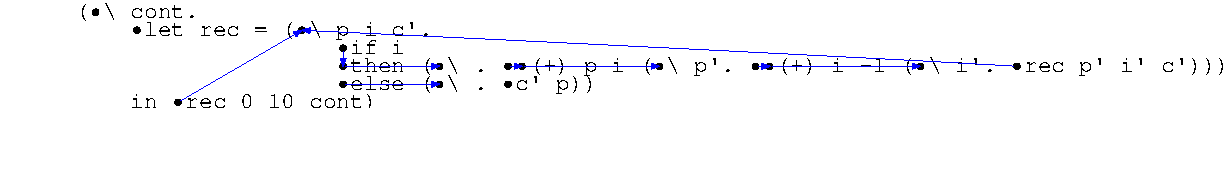
\includegraphics[width=\linewidth]{rendered-graph.pdf}%
% \end{framed}%
% \caption{The code annotated with the control cache}%
% \label{fig:ccgraph}%
% \end{figure}
% 
% After the pretty printer has laid out the code, we can gather the coordinates of all characters with code points larger or equal to U+100000 and replace them by a placeholder symbol (we chose $\bullet$). The pretty printed code is written to a PDF file using the HPDF library\cite{HPDF}, which is implemented in pure Haskell. This gives us maximal control over the positioning and allows us to render the document without padding.
% 
% To draw the arrows, we want to use the graphviz suite\cite{Graphviz} which includes several graph layout mechanisms. From the edges given by the control cache and the label coordinates from the pretty-printed code a graph description in the dot-format is generated and rendered to PDF using the \texttt{neato} command. The two PDF files are now mapped onto each other using \texttt{pdftk}\cite{pdftk}. If everything went right, the arrows will begin and end exactly at the character that replaced the label. A result is included in \vref{fig:ccgraph}.
% 
% This was just a quick experiment and serves as a proof-of-concept. Obviously, this presentation has its weakness, such as the reduced legibility of the code due to the arrows passing semi-transparently over the text.

Another conversion function is included that turns a program into the syntax used by Isabelle, to make it more convenient to define example programs in Isabelle.

\chapter{The Isabelle Formalization}
\label{chapisabelle}

The main mission of this student research project was to implement Shivers’ algorithms in the theorem prover Isabelle\citep{isabelle} and proof his main results. The main hurdles to take were
\begin{itemize}
\item representing partial functions such as the semantics functions in Isabelle within the default logic HOL, which is a logic of total functions,
\item and obtaining the fact that the set of subterms of a program is finite.
\end{itemize}

\section{Structure}

\begin{figure}
\begin{framed}
\centering
%\includegraphics{sessionGraph.pdf}
\input{sessionGraph.tex}
\end{framed}
\caption{Isabelle theories and their dependencies}
\label{fig:sessionGraph}
\end{figure}

I separated the formalizations into several files (called theories in Isabelle-speak). Their dependencies are given in \vref{fig:sessionGraph}, where squared theories contain definition, boxed theories contain the main results and theories in rounded boxes contain auxiliary definitions and lemmas. The definitional theories have directly corresponding counter-parts in the Haskell prototype. The following list gives a quick summary of their content.

\begin{description}
\setlength\parskip{0pt}
\item[CPSScheme] contains the definitions of the abstract syntax to represent the functional programs.
\item[Eval] is an implementation of the standard semantics.
\item[ExCF] is an implementation of the exact nonstandard semantics.
\item[AbsCF] is an implementation of the abstract nonstandard semantics.
\vspace{1em}
\item[ExCFSV] proves that a call cache returned by the exact nonstandard semantics is indeed a partial map.
\item[AbsCFCorrect] proves that the abstract nonstandard semantics safely approximate the exact nonstandard semantics.
\item[Computability] contains Shivers’ general treatment of equations whose least solution is computable.
\item[AbsCFComp] applies the results from the previous theory to the abstract nonstandard semantics. This step was skipped by Shivers.
\vspace{1em}
\item[Utils] is a potpourri of various lemmas not specific to our project, some of which could very well be included in the default Isabelle library.
\item[HOLCFUtils] contains generic lemmas related to the use of \isa{HOLCF}, a domain theory extension to Isabelle.
\item[CPSUtils] defines sets of subterms for \isa{CPSScheme} programs and proves their finiteness.
\item[FixTransform] transforms fixed point expressions defining two mutually recursive functions to fixed point expressions defining a single function.
\item[SetMap] contains functions and lemmas to work with set-valued maps.
\item[MapSets] defines sets of functions and sets of maps, and shows the finiteness of such maps, if their domains and ranges are finite.
\end{description}

\section{Domain theory in Isabelle}

Generally it is straight-forward to transform functional code, such as the Haskell prototype, into Isabelle. For total functions, the \isa{\isacommand{function}} package\citep{isabelle-function} provides a great deal of convenience, such as automatic termination proofs, overlapping patterns in the defining equations and mutual recursion. Unfortunately, the important functions that we would like to define, $\F$ and $\C$, are not total functions: For non-terminating programs they recurse endlessly.

The function package has some support for partial functions using the \texttt{domintros} option, which introduces a termination predicate that appears in the premises to any lemma about the functions. After having formalized the functions in that setting this turned out to be a major restriction and we looked for alternatives.

Shivers handles the issue using the machinery of domain theory, where functions defined by recursive definitions are obtained by constructing a functional on the space of function, proving that it is continues and then taking the least fixed point of the function as the desired definition. The \isa{HOLCF}-package\citep{HOLCF}, which is an extension to the standard Higher Order Logic of Isabelle, provides the necessary definitions to do domain theory in Isabelle.

A simple example for a function defined by recursion would be the function $f\colon \N \to \N$ that gives final value in the Collatz series starting with the argument:
\[
f(n) \da 
\begin{cases}
1, &\text{if } n = 1\\
f(\frac n 2), &\text{if $n$ is even} \\
f(3\cdot n + 1), &\text{otherwise}.
\end{cases}
\]
Defining this function with the \isa{\isacommand{function}} package would be very difficult, as we either had to prove that it is total, thereby proving the Collatz conjecture, or work with the inconvenient domain predicates generated by the \texttt{domintros} option.

Within \isa{HOLCF}, we can define the function $f$ as the least defined function fulfilling the above property. To be able to do so, the function space needs to have a chain-complete partial order. We therefore extend the range of the function by the special value $\bot$ to indicate undefinedness. Now f is the least fixed point $f = \text{fix}(F)$ under a functional $F\colon (\N \to \N_\bot) \to (\N \to \N_\bot)$ derived from the above specification:
\[
F(f) \da \lambda n.\ 
\begin{cases}
1, &\text{if } n = 1\\
f(\frac n 2), &\text{if $n$ is even} \\
f(3\cdot n + 1), &\text{otherwise}.
\end{cases}
\]
The least fixed point exists and is unique if $F$ is continuous, i.e.\ if it is monotonous and preserves limits of chains.

\begin{figure}
\begin{framed}
%
\begin{isabellebody}%
\def\isabellecontext{Collatz}%
%
\isadelimtheory
%
\endisadelimtheory
%
\isatagtheory
\isacommand{theory}\isamarkupfalse%
\ Collatz\ \isakeyword{imports}\ HOLCF\ \isakeyword{begin}%
\endisatagtheory
{\isafoldtheory}%
%
\isadelimtheory
\isanewline
%
\endisadelimtheory
\isanewline
\isacommand{fixrec}\isamarkupfalse%
\ f\ {\isacharcolon}{\isacharcolon}\ {\isachardoublequoteopen}nat\ discr\ {\isasymrightarrow}\ nat\ lift{\isachardoublequoteclose}\isanewline
\isakeyword{where}\ {\isachardoublequoteopen}f{\isasymcdot}n\ {\isacharequal}\ {\isacharparenleft}if\ undiscr\ n\ {\isacharequal}\ {\isadigit{1}}\ then\isanewline
\ \ \ \ \ \ \ \ \ \ \ \ \ \ \ Def\ {\isadigit{1}}\isanewline
\ \ \ \ \ \ \ \ \ \ \ \ \ else\ if\ even\ {\isacharparenleft}undiscr\ n{\isacharparenright}\ then\isanewline
\ \ \ \ \ \ \ \ \ \ \ \ \ \ \ f{\isasymcdot}{\isacharparenleft}Discr\ {\isacharparenleft}{\isacharparenleft}undiscr\ n{\isacharparenright}\ div\ {\isadigit{2}}{\isacharparenright}{\isacharparenright}\isanewline
\ \ \ \ \ \ \ \ \ \ \ \ \ else\isanewline
\ \ \ \ \ \ \ \ \ \ \ \ \ \ \ f{\isasymcdot}{\isacharparenleft}Discr\ {\isacharparenleft}{\isadigit{3}}\ {\isacharasterisk}\ undiscr\ n\ {\isacharplus}\ {\isadigit{1}}{\isacharparenright}{\isacharparenright}{\isacharparenright}{\isachardoublequoteclose}\isanewline
\isanewline
\isacommand{lemma}\isamarkupfalse%
\ {\isachardoublequoteopen}f{\isasymcdot}{\isacharparenleft}Discr\ {\isadigit{4}}{\isadigit{2}}{\isacharparenright}\ {\isacharequal}\ Def\ {\isadigit{1}}{\isachardoublequoteclose}%
\isadelimproof
\ %
\endisadelimproof
%
\isatagproof
\isacommand{by}\isamarkupfalse%
\ simp%
\endisatagproof
{\isafoldproof}%
%
\isadelimproof
%
\endisadelimproof
\isanewline
%
\isadelimtheory
%
\endisadelimtheory
%
\isatagtheory
\isacommand{end}\isamarkupfalse%
%
\endisatagtheory
{\isafoldtheory}%
%
\isadelimtheory
%
\endisadelimtheory
\end{isabellebody}%
%%% Local Variables:
%%% mode: latex
%%% TeX-master: "root"
%%% End:

\end{framed}
\caption{Function definitions with \isa{HOLCF}.}
\label{fig:collatz}
\end{figure}

\isa{HOLCF} relieves the user from the burden of transforming the recursive equations into a functional by offering the \isa{\isacommand{fixrec}} command, which is demonstrated in \vref{fig:collatz}. This command turns a recursive function definition or several mutually recursive function definitions internally into a functional, defines the function as the fixed points and proves simplification and induction lemmas for the function.

By default, no partial order is defined for $\N$, because there is more than one sensible choice. To tell the system which order to use we use the wrapper \isa{discr} for the discrete ordering, with conversion functions \isa{Discr} and \isa{undiscr}, and \isa{Lift} for the ordering with one additional element denoting bottom, with constructor \isa{Def}.

A lemma such as $f(42)=1$ would not be shown as easy as in \vref{fig:collatz} if we had used the \isa{\isacommand{function}} package with the \texttt{domintros} option, as the termination predicate had to be proven first.

Clearly, \isa{HOLCF} was the right choice to define our semantics function. In this case, the domain is a set. In Isabelle, sets over a type \isa{'a} are just functions \isa{'a\ \isasymRightarrow\ bool}. In the theory \isa{HOLCFUtils}, we therefore defined a partial order on \isa{bool}, with \isa{false\ \isasymsqsubset\ true}, to obtain the usual order on sets, where $A \sqsubseteq B \iff A \subseteq B$. For the integers, which occur as labels in the return value, contour counters and types from the syntax definition, the discrete order is defined. The arguments to the $\C$ and $\F$ functions are uncurried, i.e.\ written as one quadruple, and wrapped in \isa{Discr}. This way, all occurring types have a partial order and \isa{HOLCF} can work with them.

As mentioned before, least fixed points exists if the functional is continuous. The \isa{\isacommand{fixrec}} command hides this from the user by automatically proving continuity if the functional is defined using continuous building blocks. If this is not sufficient, an error message is shown which contains the remaining continuity goal and the user can add new rules to the set used by \isa{\isacommand{fixrec}}, named \isa{cont2cont}. In our case, continuity lemmas for booleans and sets were helpfully provided by Brian Huffman, and continuity lemmas about case expressions for our custom data types had to be written.

\section{Fixed point induction}

The main method to show results about a least fixed point is the fixed point induction, as explained on page \pageref{fixedpointinduction}. This technique was used for all main results obtained about the semantics functions. Again, \isa{HOLCF} provides some machinery to show the admissibility criterion without much effort.

A disadvantage of the fixed point induction is that it is not possible to show and use auxiliary lemmas about the function: While proving the inductive case, one does not show results for the function in question, but for an information-theoretical approximation. Thus, any previously shown results are not available. Therefore, the inductions of the auxiliary lemmas have to be intertwined in the induction of the main result.

In our case, we had to resort to this measure in the proof that the call cache returned by the exact semantics is a partial map, in theory \isa{ExCFSV}: The auxiliary lemma stated if $b$ is the contour pointed passed to $\F$ resp. $\C$, then every contour environments in the returned call cached mentions a contour counter greater or equal to $b$, if for $\F$ $b$ is strictly larger than all contour counters occurring in the arguments to $\F$ resp. for $\C$ the contour counter $b$ occurs in the contour environment passed to $C$ and is larger than all contour counters occurring in the arguments to $\C$. The main lemma just states that the call cache is a partial map, which corresponds to the predicate \isa{single-valued} of the Isabelle library. The resulting intertwined lemma, as defined in Isabelle, is shown in \vref{fig:intertwined}.
 
\begin{figure}
\begin{framed}
%
\begin{isabellebody}%
\def\isabellecontext{ExCFSV}%
\isamarkuptrue%
\isacommand{lemma}\isamarkupfalse%
\ cc{\isacharunderscore}single{\isacharunderscore}valued{\isacharprime}{\isacharcolon}\isanewline
\ \ \ \ \ \ {\isachardoublequoteopen}{\isasymlbrakk}\ {\isasymforall}b{\isacharprime}\ {\isasymin}\ contours{\isacharunderscore}in{\isacharunderscore}ve\ ve{\isachardot}\ b{\isacharprime}\ {\isacharless}\ b\isanewline
\ \ \ \ \ \ \ {\isacharsemicolon}\ {\isasymforall}b{\isacharprime}\ {\isasymin}\ contours{\isacharunderscore}in{\isacharunderscore}d\ d{\isachardot}\ b{\isacharprime}\ {\isacharless}\ b\isanewline
\ \ \ \ \ \ \ {\isacharsemicolon}\ {\isasymforall}d{\isacharprime}\ {\isasymin}\ set\ ds{\isachardot}\ {\isasymforall}b{\isacharprime}\ {\isasymin}\ contours{\isacharunderscore}in{\isacharunderscore}d\ d{\isacharprime}{\isachardot}\ b{\isacharprime}\ {\isacharless}\ b\isanewline
\ \ \ \ \ \ \ {\isasymrbrakk}\isanewline
\ \ \ \ \ \ \ {\isasymLongrightarrow}\isanewline
\ \ \ \ \ \ \ {\isacharparenleft}\ \ \ single{\isacharunderscore}valued\ {\isacharparenleft}{\isasymF}{\isasymcdot}{\isacharparenleft}Discr\ {\isacharparenleft}d{\isacharcomma}ds{\isacharcomma}ve{\isacharcomma}b{\isacharparenright}{\isacharparenright}{\isacharparenright}\isanewline
\ \ \ \ \ \ \ {\isasymand}\ {\isacharparenleft}{\isasymforall}\ {\isacharparenleft}{\isacharparenleft}lab{\isacharcomma}{\isasymbeta}{\isacharparenright}{\isacharcomma}t{\isacharparenright}\ {\isasymin}\ {\isasymF}{\isasymcdot}{\isacharparenleft}Discr\ {\isacharparenleft}d{\isacharcomma}ds{\isacharcomma}ve{\isacharcomma}\ b{\isacharparenright}{\isacharparenright}{\isachardot}\isanewline
\ \ \ \ \ \ \ \ \ \ \ \ \ \ \ {\isasymexists}\ b{\isacharprime}{\isachardot}\ b{\isacharprime}\ {\isasymin}\ ran\ {\isasymbeta}\ {\isasymand}\ b\ {\isasymle}\ b{\isacharprime}{\isacharparenright}\isanewline
\ \ \ \ \ \ \ {\isacharparenright}{\isachardoublequoteclose}\isanewline
\ \ \isakeyword{and}\ {\isachardoublequoteopen}{\isasymlbrakk}\ b\ {\isasymin}\ ran\ {\isasymbeta}{\isacharprime}\isanewline
\ \ \ \ \ \ \ {\isacharsemicolon}\ {\isasymforall}b{\isacharprime}{\isasymin}ran\ {\isasymbeta}{\isacharprime}{\isachardot}\ b{\isacharprime}\ {\isasymle}\ b\isanewline
\ \ \ \ \ \ \ {\isacharsemicolon}\ {\isasymforall}b{\isacharprime}\ {\isasymin}\ contours{\isacharunderscore}in{\isacharunderscore}ve\ ve{\isachardot}\ b{\isacharprime}\ {\isasymle}\ b\isanewline
\ \ \ \ \ \ \ {\isasymrbrakk}\isanewline
\ \ \ \ \ \ \ {\isasymLongrightarrow}\isanewline
\ \ \ \ \ \ \ {\isacharparenleft}\ \ \ single{\isacharunderscore}valued\ {\isacharparenleft}{\isasymC}{\isasymcdot}{\isacharparenleft}Discr\ {\isacharparenleft}c{\isacharcomma}{\isasymbeta}{\isacharprime}{\isacharcomma}ve{\isacharcomma}b{\isacharparenright}{\isacharparenright}{\isacharparenright}\isanewline
\ \ \ \ \ \ \ {\isasymand}\ {\isacharparenleft}{\isasymforall}\ {\isacharparenleft}{\isacharparenleft}lab{\isacharcomma}{\isasymbeta}{\isacharparenright}{\isacharcomma}t{\isacharparenright}\ {\isasymin}\ {\isasymC}{\isasymcdot}{\isacharparenleft}Discr\ {\isacharparenleft}c{\isacharcomma}{\isasymbeta}{\isacharprime}{\isacharcomma}ve{\isacharcomma}b{\isacharparenright}{\isacharparenright}{\isachardot}\isanewline
\ \ \ \ \ \ \ \ \ \ \ \ \ \ \ {\isasymexists}\ b{\isacharprime}{\isachardot}\ b{\isacharprime}\ {\isasymin}\ ran\ {\isasymbeta}\ {\isasymand}\ b\ {\isasymle}\ b{\isacharprime}{\isacharparenright}\isanewline
\ \ \ \ \ \ \ {\isacharparenright}{\isachardoublequoteclose}\isanewline
%
\isadelimproof
%
\endisadelimproof
\isanewline
\isacommand{lemma}\isamarkupfalse%
\ evalPR{\isacharunderscore}single{\isacharunderscore}valued{\isacharcolon}\isanewline%
\ \ \ \  {\isachardoublequoteopen}single{\isacharunderscore}valued\ {\isacharparenleft}{\isasymPR}\ prog{\isacharparenright}{\isachardoublequoteclose}
\end{isabellebody}%
%%% Local Variables:
%%% mode: latex
%%% TeX-master: "root"
%%% End:

\end{framed}
\caption{Intertwined fixed point inductions}
\label{fig:intertwined}
\end{figure}

\section{Finiteness of subexpressions}

For the computability proof, we need the fact that the set of subexpressions of a program is finite. This lemma, although obvious, turned out to be tricky to be proven. One complication arises from the fact that there are subexpressions of various types in a program – calls, lambdas, variables, values, labels, primitive operations – some of which are mutually recursive.

Our first approach was to define the set of subexpressions by a recursive function that runs itself for the immediate subexpressions of the argument and then inserts the argument to the set. Using the induction rule for this function, the finiteness of the resulting set is easily shown. Unfortunately, we also need lemmas about how these sets relate: If we have a lambda expression and know that it is in the set of lambdas of a program, then we need to know that the call within the lambda expression is in the set of calls of this program. Because the two sets are generated independently, this lemma required a full-fledged induction over the syntax tree. The induction rule for the mutually recursive types \isa{lambda}, \isa{call} and \isa{val} also requires special hypotheses for the occurrences of the types which are wrapped in lists, such as the list of bindings in a \isa{Let} expression. So although we are only interested in the seemingly trivial fact \isa{Lambda\ l\ vs\ c\ {\isasymin}\ lambdas\ x\ {\isasymLongrightarrow}\ c\ {\isasymin}\ calls\ x}, the complicated proof shown in \vref{fig:subexprlemma} is required. 12 such lemmas, which fortunately were all provable by only slight variations of the apply script in the figure, had to be added.

A much cleaner approach would be a combined definition of the sets of subexpressions in one \isa{\isacommand{inductive{\isacharunderscorekeyword}set}}, which could be defined by exactly the 12 lemmas mentioned above. The downside of that approach is that the finiteness of these sets turned out to be hard to come by.

Under the hood \isa{\isacommand{inductive{\isacharunderscorekeyword}set}} works very similar to \isa{\isacommand{fixrec}} as it defines the resulting set as the least fixed point of a functional. Because sets form a complete lattice, only monotonicity of the functional is required and proven automatically. Our second approach was now to create a generally applicably lemma where such a functional $F$ gives rise to a finite set. The conditions for finiteness were
\begin{itemize}
\item Monotonicity of the functional, which can be proven mechanically.
\item Finiteness preservation, i.e.\ if $S$ is finite, then $F\ S$ is also finite.
\item Descending measure of new elements. So each element $x\in F S \setminus S$ is either added unconditionally ($x\in F\ \{\}$), or there is an element $y \in S$ such that $s(x) < s(y)$ for some naturals-valued measure function $s$ (usually Isabelles \isa{size} function).
\end{itemize}
We proved this lemma but then ran into a dead end when we found out how \isa{\isacommand{inductive{\isacharunderscorekeyword}set}} treats mutually recursive sets: If sets over the types $\alpha$ and $\beta$ are to be defined, then the fixed point is a set of triples $(bool,\alpha,\beta)$. This is used to encode the direct sum $\alpha + \beta$: The boolean indicates of which type the value is, the other position in the triple is ignored. This encoding is redundant and the functional constructed by \isa{\isacommand{inductive{\isacharunderscorekeyword}set}} unfortunately happens to add an infinite number of invalid elements to the set. This does not affect the definitions, as only the valid elements are considered when defining the individual sets, but prevents this approach to finiteness from succeeding.

A third approach was suggested to us by Andreas Lochbihler. Here, subexpressions of any type are assigned a position, which is a list of natural numbers. The set \isa{Pos p} of valid positions in the program \isa{p} is defined using \isa{\isacommand{function}} and finiteness is shown easily. A function \isa{subterm} is defined, mapping each position to the corresponding subexpression. We show that the inductively defined sets of subexpressions are subsets of the range of \isa{subterm} and then thus obtained the finiteness of these sets.
 

\begin{figure}
\begin{framed}
%
\begin{isabellebody}%
\def\isabellecontext{CPSUtils}%
%
\isacommand{lemma}\isamarkupfalse%
\ \isanewline
\ \ \isakeyword{shows}\ lambdas{\isadigit{1}}{\isacharcolon}\ {\isachardoublequoteopen}Lambda\ l\ vs\ c\ {\isasymin}\ lambdas\ x\ {\isasymLongrightarrow}\ c\ {\isasymin}\ calls\ x{\isachardoublequoteclose}\isanewline
\ \ \isakeyword{and}\ {\isachardoublequoteopen}Lambda\ l\ vs\ c\ {\isasymin}\ lambdasC\ y\ {\isasymLongrightarrow}\ c\ {\isasymin}\ callsC\ y{\isachardoublequoteclose}\isanewline
\ \ \isakeyword{and}\ {\isachardoublequoteopen}Lambda\ l\ vs\ c\ {\isasymin}\ lambdasV\ z\ {\isasymLongrightarrow}\ c\ {\isasymin}\ callsV\ z{\isachardoublequoteclose}\isanewline
\ \ \isakeyword{and}\ {\isachardoublequoteopen}{\isasymforall}z{\isasymin}\ set\ list{\isachardot}\ Lambda\ l\ vs\ c\ {\isasymin}\ lambdasV\ z\ {\isasymlongrightarrow}\ c\ {\isasymin}\ callsV\ z{\isachardoublequoteclose}\isanewline
\ \ \isakeyword{and}\ {\isachardoublequoteopen}{\isasymforall}x{\isasymin}\ set\ {\isacharparenleft}list{\isadigit{2}}\ {\isacharcolon}{\isacharcolon}\ {\isacharparenleft}var\ {\isasymtimes}\ lambda{\isacharparenright}\ list{\isacharparenright}\ {\isachardot}\ Lambda\ l\ vs\ c\ {\isasymin}\ lambdas\ {\isacharparenleft}snd\ x{\isacharparenright}\ {\isasymlongrightarrow}\ c\ {\isasymin}\ calls\ {\isacharparenleft}snd\ x{\isacharparenright}{\isachardoublequoteclose}\isanewline
\ \ \isakeyword{and}\ {\isachardoublequoteopen}Lambda\ l\ vs\ c\ {\isasymin}\ lambdas\ {\isacharparenleft}snd\ {\isacharparenleft}t{\isacharcolon}{\isacharcolon}\ var{\isasymtimes}lambda{\isacharparenright}{\isacharparenright}\ {\isasymLongrightarrow}\ c\ {\isasymin}\ calls\ {\isacharparenleft}snd\ t{\isacharparenright}{\isachardoublequoteclose}\isanewline
%
\isadelimproof
%
\endisadelimproof
%
\isatagproof
\isacommand{apply}\isamarkupfalse%
\ {\isacharparenleft}induct\ rule{\isacharcolon}lambda{\isacharunderscore}call{\isacharunderscore}val{\isachardot}inducts{\isacharparenright}\isanewline
\isacommand{apply}\isamarkupfalse%
\ auto\isanewline
\isacommand{apply}\isamarkupfalse%
\ {\isacharparenleft}case{\isacharunderscore}tac\ c{\isacharcomma}\ auto{\isacharparenright}{\isacharbrackleft}{\isadigit{1}}{\isacharbrackright}\isanewline
\isacommand{apply}\isamarkupfalse%
\ {\isacharparenleft}rule{\isacharunderscore}tac\ x{\isacharequal}{\isachardoublequoteopen}{\isacharparenleft}{\isacharparenleft}a{\isacharcomma}\ b{\isacharparenright}{\isacharcomma}\ ba{\isacharparenright}{\isachardoublequoteclose}\ \isakeyword{in}\ bexI{\isacharcomma}\ auto{\isacharparenright}\isanewline
\isacommand{done}\isamarkupfalse%
%
\endisatagproof
{\isafoldproof}%
\end{isabellebody}%
%%% Local Variables:
%%% mode: latex
%%% TeX-master: "root"
%%% End:

\end{framed}
\caption{One of 12 unwieldy proofs to relate two sets of subexpressions.}
\label{fig:subexprlemma}
\end{figure}

\section{Finishing the computability proof}

As mentioned on page \pageref{shiverscomputabilty}, Shivers shows the computability only abstractly for a single recursively defined function, and leaves it to the reader to generalize this to mutually recursive function. We carried this step out in detail. To do so, we need to transform a fixed point for two functions (implemented in \isa{HOLCF} as a fixed point over a tuple) to a simple fixed point equation. The approach here works as long as both functions in the tuple have the same return type, using the equation
\[
X^A\cdot X^B = X^{A+B}.
\]

In theory \isa{FixTransform} we showed that a fixed point can be transformed using any retractable continuous function:
\[
g \circ f = \id \implies \fix(F) = g(\fix(f \circ F \circ g))
\]
and used this with the functions that convert between the tuple of functions and the combined function to transform fixed points as required. In theory \isa{AbsCFComp}, this these results are applied to $\aC$ and $\aF$ and combined with Shivers abstract computability lemmas.

\section{Cosmetics}
\label{seclayout}

We tried to follow Shivers very closely not only in substance but also in presentation. Isabelle is already very strong in generating documents from its theories that resemble common mathematics notation very closely. We employed some tricks to increase similarity with Shivers’ dissertation.

Functions in Isabelle need to have an alphanumeric name. Shivers calls his function by symbols ($\F$, $\aC$,\ldots). To achieve this, we give a the symbol a syntax translations. So the evaluation function for lambdas is called \isa{evalF}, but Isabelle also understands the code \texttt{\textbackslash<F>} which is by default set up to render as $\F$. We use the alternative symbol throughout the code and real name \isa{evalF} only appears in the definition and when referencing lemmas generated by \isa{\isacommand{function}}. 

Shivers uses some symbols that do exist as predefined isabelle symbols, e.g. $\aF$ or $\aPR$. In that case, we “invent” the symbol by writing \texttt{\textbackslash<aPR>} and adding an appropriate definition for the \LaTeX{} command \texttt{\textbackslash isasymaPR} to our document.

A similar definition is used for the power-set function used in the computability proof. Shivers denotes it by underlining the argument. This was achieved by a syntax translation \texttt{\textbackslash <\^{}ps>} and a corresponding \LaTeX{} command \texttt{\textbackslash isactrlps}, defined to be \texttt{\{\textbackslash uline \#1\}}.

In the proof about the safe approximation of $\aF$ and $\aC$, two symbols are used overloaded: The abstraction functions $|\cdot|$ and the approximation relation $\lessapprox$. This is per se not a problem, as Isabelle allows for ambiguous syntax translations. In that case, it generates more than one parse tree and picks the (hopefully unique) tree that typechecks.

Unfortunately, this does not work well in our case: There are eight concrete functions which we want to write as $|\cdot|$ and some expressions have multiple occurrences of these, causing an exponential blow-up of combinations.

Luckily, the latest development version of Isabelle contains a module by Christian Sternagel and Alexander Krauss for ad-hoc overloading, where the choice of the concrete function is done at parse time and immediately, based on the argument types. Using this system, we were able to write $|\cdot|$ and $\lessapprox$ just as Shivers did.

\section{Tool}

The most common development environment for working with Isabelle theories is ProofGeneral, an extension to the text editor Emacs. It offers conversion between Isabelle symbol strings (\texttt{\textbackslash<beta>}) and the symbol ($\beta$), allows the user to control the evaluation of the Isabelle code and shows Isabelle’s messages such as proof goals and errors.

Emacs is a relatively large and powerful editor and a great tool for the experienced user. But because the author is used to the similarly powerful editor vim, the prospect of learning Emacs just for working with Isabelle was not a nice one.

One of the alternatives is the relatively young project i3p\citep{i3p}, which provides a similar feature set based on the Netbeans frameworks and thus offers a fairly standard UI environment. Over the course of the project, we have found and reported some minor bugs and reported these to the author, who then released new versions.

A larger problem was observed with proofs involving large goal state: i3p, in contrast to ProofGeneral, reads the goal state after each command to allow the user to read earlier goal states without having to re-evaluate the theory. This is a noticeable improvement of usability. Unfortunately, it is quite expensive to print Isabelle large goal states, as they are run through various stages of syntax translations. Some theories become unbearable slow to evaluate and in some cases, we employed workarounds to avoid large goal states. But also for this case the author found a solution and the latest version of i3p now uses lazy goal states, which means that goal states are only generated by isabelle when actually displayed by i3p. The overhead for remembering the earlier goal states within Isabelle is low, thanks to the efficient sharing of values in functional languages. 


\chapter{Towards Slicing}
\label{chapslicing}


\appendix

{
\raggedright
\bibliography{root}
}
\chapter*{Erklärung}

\lettrine H{iermit} erkläre ich, Joachim Breitner, dass ich die vorliegende Studienarbeit selb\-ständig
und ausschließlich unter Verwendung der angegebenen Quellen und Hilfsmittel verfasst
habe.
\vspace{20mm}
\begin{tabbing}
\rule{4cm}{.4pt}\hspace{1cm} \= \rule{7cm}{.4pt} \\
Ort, Datum \> Unterschrift
\end{tabbing}

\end{document}
